\section{\textcite{ChenConvolutionalNeuralNetworks2017}}
Das Paper ``\citetitle*{ChenConvolutionalNeuralNetworks2017}'' von \citeauthor*{ChenConvolutionalNeuralNetworks2017} betrachtet die Dokumentensegmentierung als ein ``pixel labeling problem''. 
Aber eines der größten Probleme bei der Verarbeitung von Dokumentenseiten die Größe der Scanbilder.
Genauer gesagt modelieren \citeauthor{ChenConvolutionalNeuralNetworks2017}  die Segmentierung als ein Superpixelklassifizerungsproblem.
Die Bilder im HisDB-Datenset sind mit einer Auflösung von \(4872 \times 6496\) wesentlich größer als andere Datensets.\qq{Welche?}
Um den Prozess zu beschleunigen werden nicht alle Pixel sondern nur etwa 3000 Pixelcluster klassifiziert. 

\subsection{Vorverarbeitung}
\citeauthor{ChenConvolutionalNeuralNetworks2017} skalieren alle Bilder mit einem Faktor von  \(2^{-3}\) und wenden dann den Superpixelalgorithmus SLIC (simple linerar iterative clustering) an \parencite{AchantaSLICSuperpixels2010} um die Dokumentenseiten in Superpixel einzuteilen.
Ein \(28 \times 28\)-Bereich um das Zentrum des Superpixel wird dann mithilfe eines CNN
klassifiziert. Diese Klassifizierung wird dann allen Pixel innerhalb des Superpixels zugewiesen.

\begin{figure}
    \centering
    \caption{Die SLIC-Pixelgrenzen sind in rot dargestellt }
    \label{fig:slic_parameters}
    \subfloat[ \(m = 0.1\)]{
        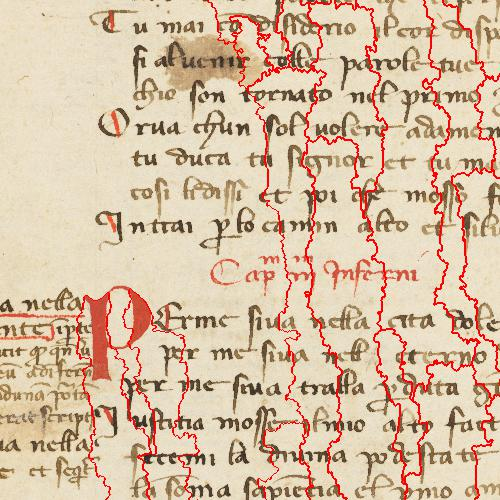
\includegraphics[width=0.24\textwidth]{figures/img/mark_boundaries_m0.jpg}
    }
    \subfloat[\(m = 1\)]{
        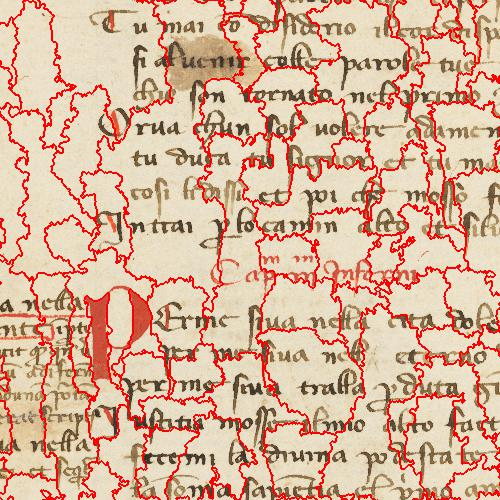
\includegraphics[width=0.24\textwidth]{figures/img/mark_boundaries_m1.jpg}
    }
    \subfloat[\(m = 10\)]{
        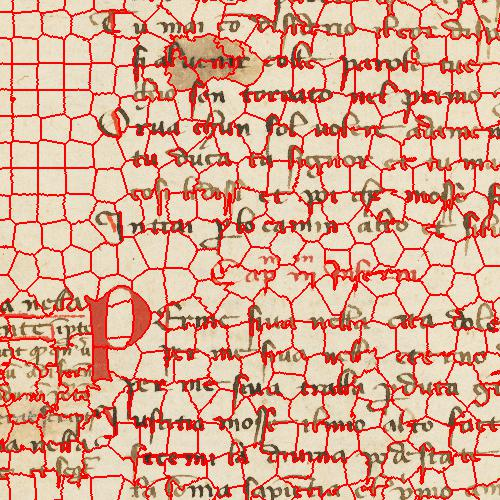
\includegraphics[width=0.24\textwidth]{figures/img/mark_boundaries_m10.jpg}
    }
    \subfloat[\(m = 100\)]{
        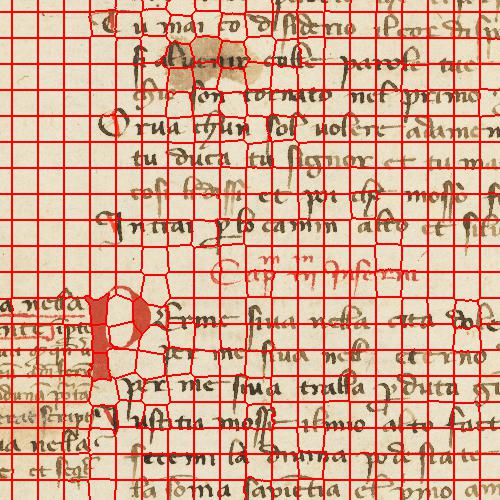
\includegraphics[width=0.24\textwidth]{figures/img/mark_boundaries_m100.jpg}
    }
\end{figure}

\citeauthor{AchantaSLICSuperpixelsCompared2012} stellen später zwei wichtige Erweiterungen vor:
Normalisierung des Distanzmaßes und Adaptive-SLIC.

\citeauthor{ChenConvolutionalNeuralNetworks2017a} nennen keine Details zur Wahl
der Superpixel-Parameter, verweisen aber auf eine frühere Studie die sich mit unterschiedlichen 
Superpixel verfahren beschäftigt \parencite{ChenPageSegmentationHistorical2016}.
Die Studie versucht einen Autoencoder (siehe \ref{sec:autoencoder}) zu trainieren auf Basis von Superpixeln und vergleicht dabei den Einfluss von unterschiedlichen Superpixel-Methoden. Die veröffenlichen Ergebniss zeigen aber nur die Performanz im Bezug
auf die Zahl der Cluster \(n \in \left\{10^3, 50^3, 100^3, 200^3\right\}\) und dem Skalierungsfaktor \(\alpha \in \left\{2^{-2}, 2^{-3}\right\}\)
\qq{adaptive slic}
\qq{Problem gt zu treffen}

\section{Netzwerk-Architektur}
\citeauthor{ChenConvolutionalNeuralNetworks2017a} beschreiben die Struktur
des CNN als \(28 \times 28 \times 1 - 26 \times 26 \times 4 - 100 - M\).

Während des Trainings wird das Ground-truth Label des Zentrumpixels als Label für den Superpixel verwendet.

\section{Training}

\section{Nachverarbeitung}